% Shared paper body, included identically by both main.tex (final/camera-ready) and
% main_review.tex (anonymized review mode). Edit ONLY this file for content changes -- editing the
% body in one wrapper and not the other would silently desync the two submission versions.
% Revision round 2 (T21, 2026-09-28): restructured per research/paper/review_round1 and
% research/paper/T21_REVISION_LOG.md; every number traces to research/results (see the log).

\begin{abstract}
Natural-language shell assistants are usually built by generation. We audit a published closed-set
alternative: a BM25 retriever over 279 Windows commands that shows its user a confidence and runs the
chosen command on Enter. Its confidence is no better than a constant forecaster, and wrong answers
average 86\% confidence. With nested cross-validation on two benchmark versions (the second adds 59
out-of-scope and ambiguous queries) and 25 verbatim-copy controls excluded, three results hold.
Isotonic recalibration cuts the shipped confidence's expected calibration error by 79\% on both
versions, to about the noise floor of a perfectly calibrated forecaster; Platt scaling and histogram
binning do about as well. A tuned rejection threshold on the shipped score rejects 46 of 50
out-of-scope requests, where the fixed rule rejects 17 and a hybrid lexical--dense detector 34. The
hybrid's confidence ranks its own errors better than the shipped one, but its accuracy gain is
statistically fragile, and both systems sometimes return destructive commands for benign requests. All
analyses are exploratory; a two-annotator label study is under way.
\end{abstract}

\section{Introduction}

Natural-language shell assistance can lower the barrier to command-line tools, but a wrong command can
destroy data. Research since NL2Bash \citep{lin-etal-2018-nl2bash} has mostly generated commands: neural
translation (the NLC2CMD competition, \citealp{agarwal2021nlc2cmd}), then large language model (LLM)
systems (NL2SH; \citealp{westenfelder2025nl2sh}), most recently trained with reinforcement learning on
static-analysis rewards (BashCoder-R1; \citealp{yu2026bashcoderr1}). Retrieval over a fixed command list is an
older alternative that NLC2CMD also tested \citep{agarwal2021nlc2cmd} and ShellFusion developed
\citep{zhang2022shellfusion}. It cannot invent a command, and a small lexical retriever runs offline and
deterministically, so no query leaves the user's machine and every answer can be traced to a vetted record;
the price is coverage.

We audit one such system as it is published: TermAssist, an npm package that maps a query to one of 279
Windows commands with BM25 \citep{robertson2009bm25}, prints the command with a confidence percentage,
refuses below 30\%, and runs the pre-filled, editable command when the user presses Enter (\S\ref{sec:system}).
The printed confidence is the only reliability signal a user gets, and our reproduction of the published
baseline found it frequently confidently wrong. We therefore ask: \emph{how reliable is the confidence of a
shipped closed-set command retriever, and what do post-hoc recalibration, a tuned rejection threshold, and a
hybrid lexical--dense retriever each contribute?}

\paragraph{Contributions.} (1) An audit of a published tool's confidence: it is no better than a constant
forecaster, wrong answers average 86\% confidence, and some wrong answers are destructive commands. (2) An
attribution of what fixes what, under nested cross-validation on two benchmark versions with verbatim-copy
controls excluded: standard recalibration fixes the confidence level, a tuned threshold on the shipped score
handles out-of-scope requests, and a hybrid retriever (a research prototype, not part of the package) mainly
improves how confidence ranks the system's own errors; its accuracy gain is fragile. (3) Evaluation practice for
small closed-set benchmarks: tie-aware selective-prediction metrics, a noise floor and no-skill reference for
calibration, detection compared at matched operating points, and disclosure of every null and fragile result.

\section{Related Work}

\paragraph{Natural language to shell.} NL2Bash \citep{lin-etal-2018-nl2bash} paired English descriptions with
Bash commands. The NLC2CMD competition \citep{agarwal2021nlc2cmd} scored each prediction by utility and flag
overlap, weighted by the confidence the system submitted, so confident wrong answers were penalized; one
entry used TF-IDF retrieval with a logistic-regression model that lowered confidence on likely-wrong
predictions, and came within 12\% of the best system. ShellFusion \citep{zhang2022shellfusion} retrieves
commands from question-answer posts and re-ranks them against manual pages; DocPrompting
\citep{zhou2023docprompting} retrieves documentation, including tldr pages, before generating code; Project
CLAI \citep{agarwal2020clai} treats the command line as an environment for AI agents. NL2SH
\citep{westenfelder2025nl2sh} improves LLM translation with parsing and constrained decoding, and QuoteBench
\citep{li2026quotebench} shows that matched execution scores can hide command-path failures. We run no
generative system, so our comparison with generation is conceptual.

\paragraph{Reliability.} We draw on calibration \citep{guo2017calibration,naeini2015ece}, post-hoc
recalibration \citep{zadrozny2002isotonic,platt2000probabilistic,zadrozny2001binning}, selective classification
and its risk-coverage metrics \citep{geifman2017selective,geifman2019aurc,traub2024overcoming}, and out-of-distribution (OOD) detection
from confidence scores \citep{hendrycks2017baseline}. The closest task framing is intent classification with
out-of-scope queries \citep{larson-etal-2019-evaluation}; the closest methods are learned calibrators for
abstention under domain shift \citep{kamath-etal-2020-selective} and confidence estimation for mapping language to
programs \citep{dong-etal-2018-confidence}. In text-to-SQL, selective classifiers mostly catch irrelevant questions
rather than wrong queries \citep{somov2025texttosql}, which our out-of-scope breakdown echoes (\S\ref{sec:ood}).
Within our targeted search (Limitations), natural-language-to-shell retrieval work has not evaluated the calibration of a
deployed tool's confidence, tie-aware selective prediction, or out-of-scope rejection with its false-rejection
cost; to our knowledge, that combination is what is new here, not any single method.

\section{System and Benchmark}
\label{sec:system}

\paragraph{The published tool.} Queries are tokenized (lowercase, punctuation stripped, 10-word stopword list)
and scored with BM25 ($k_1=1.2$, $b=0.75$) over each record's intent, category and description, plus a flat
$+15$ bonus when the query nearly matches an intent. Confidence is $\min(\mathrm{round}(s/8\times100),100)$ for
top score $s$, and is 0 when $s<2.0$. The command-line tool prints the top command with ``confidence: $N$\%'',
refuses when $N<30$, and otherwise opens an editable prompt pre-filled with the command, which runs (in
PowerShell on Windows) when the user presses Enter; no risk level is shown. Retrieval is local; an optional
query-sync feature is off by default. Our evaluation counts a query as answered when $s\geq2.0$; no benchmark
query scores between 2.0 and 2.4, so this makes the same decisions as the 30\% rule. We reproduced the published
outputs exactly (0/150 mismatches). Mean latency was 3.3\,ms in one run on one machine, an indicative figure.

\paragraph{Corpus.} 431 records, of which 279 are visible on Windows (145 cross-platform, 134
Windows-specific), each a distinct intent. The records were checked by script rather than one by one, and a
few Windows-visible records are Linux commands (e.g., \texttt{sudo reboot}).

\paragraph{Benchmark.} v0.1 has 150 hand-adjudicated queries of 9 types, labeled CORRECT (119), AMBIGUOUS
(14), OOD (15; here, out-of-scope requests that no record serves) or NEEDS\_CORRECTION (2), with a risk level for the
gold command. All 25 \emph{canonical} queries repeat a corpus intent verbatim and every system answers them, so
we treat them as positive controls and exclude them from headline figures. v0.2 contains all of v0.1 plus 35
out-of-scope and 24 ambiguous queries, so the versions share their 121 answerable queries and are not
independent. The new queries were drafted and adjudicated by an AI agent under human direction; all 35
out-of-scope drafts were kept unchanged, and their top-1 BM25 score and dense similarity were then checked to be
low (maximum 7.39 and 0.31). Seventeen of the 24 new ambiguous queries are single tool or category names
(``grep'', ``pip''); nine of v0.1's 14 are too. Public natural-language-to-Bash benchmarks target Linux commands and do not
map onto this Windows corpus, so we did not use them. Three items have gold commands outside the Windows corpus
(TA-B145, TA-B149, TA-B187); they lower every system's non-OOD accuracy by at most 2 of 159 queries and change no
comparison. One partially independent reviewer, shown only the query text, re-labeled a stratified sample of 14
AI-authored queries: Cohen's $\kappa=0.63$ \citep{cohen1960coefficient}, below our 0.7 target. The reviewer
agreed with all 8 out-of-scope labels (7 everyday requests and one far-from-corpus computing task, none a terminal
task) and disagreed on 3 of 6 ambiguous ones. A
two-annotator study with a written codebook is under way.

\section{Methods}
\label{sec:methods}

\paragraph{What is compared.} (i) The shipped confidence, before and after post-hoc recalibration. (ii) Three
out-of-scope rules: the shipped fixed rule ($s<2.0$), a threshold on the shipped score $s$ tuned on development
folds, and the hybrid detector. (iii) Three retrievers: BM25, dense retrieval with a 384-dimensional MiniLM
sentence encoder (\texttt{all-MiniLM-L6-v2}; \citealp{wang2020minilm,reimers-gurevych-2019-sentence}), and a hybrid
that min-max normalizes both score lists over each query's candidates and ranks by
$\alpha\,\mathrm{BM25}_{\mathrm{norm}}+(1-\alpha)\,\mathrm{dense}_{\mathrm{norm}}$. The hybrid's confidence is
its fused top-1 score, which equals 1 whenever the two retrievers agree on the top command; its detector rejects
when that score falls below a threshold. Appendix~\ref{app:spec} gives the full specification.

\paragraph{Protocol.} Five folds (seed 42, stratified by label; Split A). For each test fold, $\alpha$ (grid
0.0--1.0, maximizing non-OOD accuracy), the detector thresholds (maximizing F1) and the calibrators are chosen
on the other four folds and applied once. There is no inner split; each query's hybrid score uses the $\alpha$
chosen for its own fold ($\alpha\in\{0.3,0.5\}$ throughout). The features for the two detectors were chosen by
inspecting class means on the full data, a disclosed leak. A second split groups queries by intent (Split B),
which checks for tuning leakage across intents but cannot test unseen commands, since the corpus always holds the
gold intent (Appendix~\ref{app:secondary}).

\paragraph{Metrics and statistics.} Expected calibration error (ECE) uses 10 equal-width bins
\citep{naeini2015ece,guo2017calibration}; we also report equal-mass and sweep estimates, a noise floor (the ECE of a
perfectly calibrated forecaster with the same confidences and $n$, simulated), and Brier skill
\citep{brier1950verification} against an out-of-fold no-skill forecaster that predicts the development base rate.
Confidence often ties at its maximum (64\% of the hybrid's and 73\% of the shipped values on v0.1), so
risk-coverage curves use expected risk under a random order within ties and are summarized by the area under them (AURC; \citealp{geifman2019aurc}) and the area under the
generalized risk-coverage curve (AUGRC; \citealp{traub2024overcoming}); the area under the receiver
operating characteristic curve (AUROC) for separating right from wrong answers by confidence, which we call
correctness AUROC, measures ranking alone. Accuracy differences use the exact McNemar test \citep{mcnemar1947note}, proportions
Wilson intervals \citep{wilson1927probable}, and effects paired percentile bootstraps (10,000 resamples, seed 42),
which are not dual to the exact test. A family of four comparisons per version (accuracy vs.\ BM25 and vs.\ dense,
out-of-scope rejection, hybrid ECE reduction) is Holm-corrected \citep{holm1979simple}; it was fixed after the raw
results were seen, so \emph{all significance statements are exploratory}.

\section{Results}
\label{sec:results}

Table~\ref{tab:claims} summarizes every claim; the population throughout is non-control queries unless stated.

\begin{table*}[t]
  \centering
  \small
  \setlength{\tabcolsep}{4pt}
  \begin{tabular}{@{}p{0.32\linewidth}p{0.225\linewidth}p{0.225\linewidth}p{0.14\linewidth}@{}}
    \toprule
    \textbf{Claim} & \textbf{v0.1} & \textbf{v0.2} & \textbf{Status} \\
    \midrule
    Shipped confidence: ECE before $\to$ after isotonic & .323$\to$.069; $-$79\% [44, 84] & .293$\to$.063; $-$79\% [52, 87] & robust \\
    Shipped confidence: Brier skill vs.\ no-skill, raw / recalibrated & $-$.23 [$-$.45, .01] / .20 [.04, .36] & $-$.06 [$-$.26, .15] / .33 [.19, .46] & robust \\
    Hybrid confidence: ECE reduction (Holm-adjusted $p$, controls incl.) & $-$67\% [43, 83] ($p$=.0004) & $-$81\% [62, 86] ($p$=.0003) & robust \\
    Out-of-scope rejected: fixed rule / tuned threshold / hybrid detector & 4 / 10 / 7 of 15 & 17 / 46 / 34 of 50 & threshold, not hybrid \\
    False rejections of non-OOD: fixed / tuned / hybrid & 0 / 9 / 6 of 135 & 0 / 20 / 11 of 159 & cost of tuning \\
    Out-of-scope AUROC: shipped score minus hybrid feature & +.095 [.005, .208] & +.063 [.015, .119] & robust \\
    Hybrid minus shipped AURC (tie-aware) & $-$.115 [$-$.177, $-$.054] & $-$.075 [$-$.126, $-$.024] & robust \\
    Hybrid minus shipped correctness AUROC & +.099 [.008, .190] & +.058 [$-$.001, .118] & weak on v0.2 \\
    Accuracy, hybrid minus BM25 (pp; Holm-adj.\ $p$) & +6.4 [1.8, 10.9] (.047) & +4.5 [0.7, 9.0] (raw .070) & fragile \\
    Accuracy, hybrid minus dense (pp; Holm-adj.\ $p$) & +5.5 [0.0, 11.8] (.292) & +8.2 [2.2, 14.2] (.025) & fragile \\
    \bottomrule
  \end{tabular}
  \caption{Claims with 95\% bootstrap intervals, non-control queries unless stated (``controls incl.''). Status
  ``robust'' means the interval excludes zero on both versions; ``fragile'' means the result depends on a few
  queries (Appendix~\ref{app:secondary}). Out-of-scope rows use all queries of each version.}
  \label{tab:claims}
\end{table*}

\paragraph{The shipped confidence.} The published baseline answers 67.3\% of v0.1's 150 queries correctly, yet its
49 wrong answers carry a mean confidence of 86\%, and 44.9\% of them are shown at 100\%. Its ECE (0.323 on v0.1,
0.293 on v0.2, controls excluded) is five to six times the noise floor of a perfectly calibrated forecaster at this size
(0.064 and 0.050), and its Brier score is no better than predicting the base rate for every query (skill $-0.23$
and $-0.06$, intervals including zero). A heuristic score such as $s/8$ capped at 100\% is not expected to be
calibrated; what the audit adds is how far off it is, and that the tool shows it to users as a percentage.

\paragraph{Recalibration.} Isotonic regression fit on development folds lowers the shipped confidence's ECE to
0.069 on v0.1 and 0.063 on v0.2, a 79\% reduction on both versions and within the noise floor's 95th percentile
(0.105 and 0.080); equal-mass and sweep estimates agree. Brier skill becomes positive (0.20 and 0.33, intervals
excluding zero), so the recalibrated number carries information about correctness. Platt scaling and histogram
binning reduce ECE by similar amounts with overlapping intervals, so the gain does not depend on the method. The
hybrid's own confidence behaves the same way: raw, it is significantly worse than the no-skill forecaster; after
recalibration its ECE falls 67\% and 81\%, with residual miscalibration above the noise floor on v0.1. The
pre-named comparison in the Holm family is this hybrid reduction, with controls included, and it survives
correction on both versions (Table~\ref{tab:holm}). Recalibration changes the number shown, not the answer or its
ranking: correctness AUROC even drops slightly (hybrid, v0.1: 0.858 to 0.804), because each fold gets its own map.

\paragraph{Out-of-scope requests.}
\label{sec:ood}
The shipped fixed rule rejects 17 of v0.2's 50 out-of-scope requests. The hybrid detector rejects 34, which
survives Holm correction (adjusted $p=0.00006$), at a cost of 11 false rejections among 159 in-scope queries,
three of which the hybrid had answered correctly. But the gain comes from the threshold, not the hybrid: the
shipped score itself separates out-of-scope requests better than the hybrid's fused score (AUROC 0.963 vs.\ 0.900
on v0.2, 0.950 vs.\ 0.855 on v0.1), and a threshold on the shipped score tuned exactly like the detector rejects
46 of 50 (McNemar $p=0.004$ against the detector) at 20 false rejections ($p=0.093$). On v0.1 the tuned threshold
rejects 10 of 15 and the detector 7 ($p=0.25$). By kind of request (labels assigned by an AI assistant, unchecked),
the detector rejects 25 of 34 everyday non-computing requests, 4 of 5 far-from-corpus computing tasks, the one
nonsensical request, and 4 of the 10 terminal tasks the corpus does not cover. One caveat favors the shipped score:
the added out-of-scope queries were checked to have low raw BM25 scores, and the tuned thresholds (6.5--7.2) sit just
below their 7.39 maximum. The detector's gain is nevertheless the same on the 15 keyword-verified v0.1 queries as on
the 35 added ones (+33.3 vs.\ +34.3 points). (The same 15 queries give $p=0.25$ in the v0.1 run and $p=0.0625$ in
the v0.2 run because each run tunes its own thresholds.)

\paragraph{What the hybrid adds.} The hybrid's confidence ranks its own errors better than the shipped confidence:
tie-aware AURC and AUGRC are lower on both versions with intervals excluding zero (Table~\ref{tab:claims}), and
correctness AUROC is higher, though on v0.2 without controls its interval just includes zero. At 50\% coverage, which
lies inside the maximum-confidence tie block, the hybrid's expected error on all 150 v0.1 queries is 8.3\% (0--10.7\%
depending on how ties are ordered). Its accuracy gain is consistent in size but not established (Table~\ref{tab:acc}): over BM25 it
gains 6.4 points on v0.1 (exact $p=0.0156$, Holm-adjusted 0.047) and 4.5 on v0.2 ($p=0.070$), resting on 7 and 8
discordant queries, and one bare keyword (``system'') decides the v0.2 test. Its advantage over dense retrieval on
v0.2 depends on three bare-keyword queries (Appendix~\ref{app:secondary}). Grouping folds by intent leaves accuracy
unchanged and weakens calibration somewhat (Appendix~\ref{app:secondary}).

\begin{table}[t]
  \centering
  \small
  \setlength{\tabcolsep}{4pt}
  \begin{tabular}{@{}lrr@{}}
    \toprule
    \textbf{System} & \textbf{v0.1} & \textbf{v0.2} \\
    \midrule
    BM25 (shipped) & 72/110 (65.5) & 95/134 (70.9) \\
    Dense          & 73/110 (66.4) & 90/134 (67.2) \\
    Hybrid         & 79/110 (71.8) & 101/134 (75.4) \\
    \bottomrule
  \end{tabular}
  \caption{Non-OOD accuracy (hits/queries, \%), canonical controls excluded. Every system also answers all 25
  controls correctly (Appendix~\ref{app:secondary}).}
  \label{tab:acc}
\end{table}

\paragraph{Risky wrong answers.} The case that motivates the audit does occur (Table~\ref{tab:risk}). Classifying each
\emph{returned} command with a deterministic rule-based risk classifier, both systems return a few wrong answers whose
command is high or critical risk: ``open the config file'' returns \texttt{winget uninstall package-name --purge}
from both systems, and ``change the file permissions'' returns an ownership change at maximum confidence. On v0.2 the
hybrid also maps the bare query ``system'' to \texttt{sudo shutdown -h now} and the everyday request ``teach me how to
play guitar'' to an elevated PowerShell. The full hybrid pipeline (margin plus out-of-scope rejection) blocks 3 of its
6 such answers on v0.2, including the two out-of-scope requests, but not the config, permissions or ``system'' answers. The classifier itself is scored against the benchmark's own risk labels
(gold commands of all non-OOD queries with a gold command: 125 in v0.1): it flags 19 of 20 high- or critical-risk commands in
v0.1 and misses \texttt{git checkout -{}- .}, which discards uncommitted work (1/20, Wilson 95\% CI [0.9, 23.6]\%); v0.2
adds two misses that trace to inconsistent labels (3/22). We therefore make no safety claim. On the 15 benchmark
queries whose gold commands can run safely in a sandbox, all gold commands and 14 of 15 hybrid answers executed
successfully.

\begin{table}[t]
  \centering
  \small
  \setlength{\tabcolsep}{3pt}
  \begin{tabular}{@{}lrrrr@{}}
    \toprule
    & \multicolumn{2}{c}{\textbf{v0.1}} & \multicolumn{2}{c}{\textbf{v0.2}} \\
    & Shipped & Hybrid & Shipped & Hybrid \\
    \midrule
    Answered                 & 146 & 150 & 192 & 209 \\
    High/critical returned   & 20  & 23  & 21  & 26 \\
    \quad of which wrong     & 2   & 3   & 2   & 6 \\
    \quad \quad at max.\ conf. & 1 & 1 & 1 & 1 \\
    \bottomrule
  \end{tabular}
  \caption{Returned commands the rule-based classifier rates high or critical risk, how many are wrong answers, and how
  many of those are shown at the system's maximum confidence band (shipped: 100\%; hybrid: fused score 1.0). The
  classifier misses at least one destructive command, so counts are lower bounds.}
  \label{tab:risk}
\end{table}

\section{Discussion}

For a shipped closed-set assistant the three problems separate cleanly. The displayed confidence was the weakest
part, and standard recalibration on held-out labels repairs most of it; the number a user sees can become
informative without changing the system. Out-of-scope rejection needed a better threshold, not a new retriever: the
shipped score, thresholded well, did better than the hybrid detector, at the cost of more refused in-scope queries,
a trade-off that should be set by the relative cost of a wrong command and a refusal. The hybrid's value lies in
ranking its own errors, which matters for abstention, while its accuracy gain is too small for this benchmark to
establish \citep{card2020littlepower}. For users of a tool that runs a command on Enter, the risky wrong answers
suggest a further safeguard independent of calibration: showing the risk level and asking for confirmation, or using
PowerShell's \texttt{-WhatIf}, before destructive commands.

\section{Conclusion}

A published natural-language command retriever shows its users a confidence that is no better than a constant
forecaster. Post-hoc recalibration fixes most of that on both benchmark versions, a tuned threshold on the shipped
score handles out-of-scope requests better than a hybrid detector, and the hybrid mainly improves how confidence
ranks its own errors; its accuracy gain and its advantage over dense retrieval are fragile. Next steps, in order:
finish the two-annotator label study and release a corrected benchmark; confirm the findings with an analysis
specified in advance; add answerable and terminal-task out-of-scope queries judged by people; build an independent
safety set; and study whether calibrated confidence and risk prompts change what users run.

% Invisible marker: build.sh reads its page number to check the 8-page limit. Per the ACL formatting
% guidelines, the Limitations and Ethical Considerations sections below come after the conclusion and do
% not count toward the page limit, so the marker sits at the end of the conclusion. Keep it here.
\label{endofbody}

\section*{Limitations}

\begin{itemize}
  \item \textbf{Small, dependent, partly AI-authored benchmark.} 150 and 209 queries, the second containing the first;
  59 queries drafted by an AI agent, whose labels were checked only by one partially independent reviewer
  ($\kappa=0.63$, $n=14$); the two-annotator study has no results yet. Three items have gold commands outside the
  corpus. Queries were written by the authors and an AI agent, not collected from users, so calibration and
  out-of-scope rates depend on this mix.
  \item \textbf{Exploratory statistics.} Every analysis was specified after results were seen, including the Holm
  family, the controls exclusion, the matched operating points and the sensitivity subsets. Accuracy tests rest on
  7--8 discordant queries. Results come from one fold partition (seed 42).
  \item \textbf{Out-of-scope evidence.} Only 10 out-of-scope queries are terminal tasks outside the corpus; the kind
  labels are AI-assigned; the added queries were checked with raw retrieval scores; and detector features were chosen
  on the full data.
  \item \textbf{Scope.} One tool, one platform (Windows; results depend on the platform-filtered corpus), 279 commands,
  one small sentence encoder and one fusion rule, exact-match scoring against gold commands, and single-machine
  latencies. No generative system, user study, or public benchmark is evaluated.
  \item \textbf{Safety.} The risk classifier is scored against the benchmark's own labels, two of which are
  inconsistent, and misses at least one destructive command; functional evaluation covers 15 queries and treats exit
  code 0 as success.
  \item \textbf{Literature.} Our search was targeted (natural-language-to-shell generation and retrieval, calibration,
  selective prediction, out-of-scope detection); the novelty claim is limited to the combination evaluated here.
\end{itemize}

\section*{Ethical Considerations}

The published tool runs the command it retrieves when the user presses Enter, and our results show it can offer a
destructive command for a benign request, sometimes at maximum confidence. We report these cases rather than a safety
claim, and recommend that such tools show a risk level and require explicit confirmation for high-risk commands. This
study does not change the published package, so its findings apply to current users. No command was run on a user's
system: functional evaluation ran in disposable sandboxed directories. We disclose that part of the benchmark was
written by an AI agent and that our own label check fell below target. Code, benchmark files, result files and a
reproduction guide will be released with the camera-ready version; they are withheld from the review version for
anonymity.

\bibliography{references}

\appendix

\section{System Specification}
\label{app:spec}

\begin{table*}[t]
  \centering
  \small
  \setlength{\tabcolsep}{4pt}
  \begin{tabular}{@{}p{0.2\linewidth}p{0.76\linewidth}@{}}
    \toprule
    \textbf{Component} & \textbf{Definition} \\
    \midrule
    Dense encoder & \texttt{Xenova/all-MiniLM-L6-v2}; each record embedded as ``Intent / Description / Category / Platform'' text; cosine similarity. \\
    Fusion & Per query, BM25 (with bonus) and cosine scores are min-max normalized over all 279 candidates; score $=\alpha\,\mathrm{BM25}_{\mathrm{norm}}+(1-\alpha)\,\mathrm{dense}_{\mathrm{norm}}$; top-1 is the argmax. \\
    $\alpha$ & Grid $\{0.0,0.1,\dots,1.0\}$; maximizes non-OOD accuracy on the four development folds; ties go to 0.5. Selected: v0.1 0.3, 0.3, 0.3, 0.3, 0.5; v0.2 0.5 in every fold. \\
    Hybrid confidence & Fused top-1 score (1.0 when the BM25 and dense top-1 coincide). \\
    Margin, entropy & Top-1 minus top-2 fused score among the top 10; Shannon entropy of the top-10 scores shifted to a minimum of 0 and normalized, divided by $\log_2 10$. \\
    Out-of-scope detector & Reject if the fused top-1 score is below a per-fold threshold maximizing F1 on development folds (v0.1 0.833--0.895; v0.2 0.884--0.925). \\
    Tuned shipped threshold & Same protocol on the shipped top score $s$ (v0.1 5.42--6.19; v0.2 6.50--7.20). \\
    Ambiguity detector, A4, A5 & Flag if margin is below an F1-maximizing threshold; A4 abstains on that flag, A5 on A4's flag or the out-of-scope detector. \\
    Calibrators & Isotonic regression (pooled adjacent violators), Platt scaling, histogram binning (10 bins); fit on development folds only. \\
    \bottomrule
  \end{tabular}
  \caption{Specification of the research system (the hybrid is a research prototype, not part of the published tool).}
  \label{tab:spec}
\end{table*}

\section{Secondary Analyses}
\label{app:secondary}

\paragraph{Holm family.} Table~\ref{tab:holm} gives the pre-named family, computed with the canonical controls
included; the controls never enter discordant pairs, so accuracy $p$-values are the same without them. The
calibration $p$ is a bootstrap bound (one-sided, resolution $10^{-4}$), so its Holm value is also a bound.

\begin{table}[t]
  \centering
  \small
  \setlength{\tabcolsep}{3pt}
  \begin{tabular}{@{}llrrc@{}}
    \toprule
    \textbf{Ver.} & \textbf{Comparison} & \textbf{Raw $p$} & \textbf{Holm} & \textbf{Sig.} \\
    \midrule
    v0.1 & Acc., hybrid vs. BM25 & 0.0156 & 0.0469 & \textbf{Yes} \\
    v0.1 & Acc., hybrid vs. dense & 0.1460 & 0.2920 & No \\
    v0.1 & OOD rej., tuned vs. base & 0.25 & 0.2920 & No \\
    v0.1 & Calib. ECE reduction & $\leq$0.0001 & $\leq$0.0004 & \textbf{Yes} \\
    v0.2 & Acc., hybrid vs. BM25 & 0.0703 & 0.0703 & No \\
    v0.2 & Acc., hybrid vs. dense & 0.0127 & 0.0255 & \textbf{Yes} \\
    v0.2 & OOD rej., tuned vs. base & 0.000015 & 0.00006 & \textbf{Yes} \\
    v0.2 & Calib. ECE reduction & $\leq$0.0001 & $\leq$0.0003 & \textbf{Yes} \\
    \bottomrule
  \end{tabular}
  \caption{Holm-corrected family ($\alpha=0.05$; exploratory). ``OOD rej., tuned vs.\ base'' is the hybrid detector
  against the shipped fixed rule. Accuracy $p$ are two-sided exact McNemar; the calibration $p$ is one-sided.}
  \label{tab:holm}
\end{table}

\paragraph{Bare-keyword sensitivity.} Dropping single-token ambiguous queries (a rule stated before the subset results
were computed, though the full-benchmark result was known) leaves the BM25-to-hybrid gain at $+4.9$ to $+5.8$ points,
each subset 7--0 in discordant queries, but the v0.2 hybrid-over-dense advantage falls to raw $p=0.057$ without the new
bare-keyword queries and $p=0.227$ on answerable queries only; the calibration gain is unchanged (Table~\ref{tab:sens}).

\begin{table*}[t]
  \centering
  \small
  % AUTO-GENERATED by research/experiments/generate_sensitivity_table.js -- do not edit by hand.
\begin{tabular}{@{}llrccr@{}}
    \toprule
    \textbf{BM} & \textbf{Evaluated on} & \textbf{n} & \textbf{BM25$\to$Hyb.} & \textbf{Dense$\to$Hyb.} & \textbf{ECE red.} \\
    \midrule
    v0.1 & all queries & 135 & +5.2 (0.016) & +4.4 (0.146) & 80\% \\
    v0.1 & w/o 9 bare-keyword & 126 & +5.6 (0.016) & +4.8 (0.146) & 80\% \\
    v0.2 & all queries & 159 & +3.8 (0.070) & +6.9 (0.013) & 77\% \\
    v0.2 & w/o 17 new bare-keyword & 142 & +4.9 (0.016) & +5.6 (0.057) & 81\% \\
    v0.2 & w/o all 26 bare-keyword & 133 & +5.3 (0.016) & +6.0 (0.057) & 84\% \\
    v0.1/v0.2 & answerable only & 121 & +5.8 (0.016) & +4.1 (0.227) & 78/81\% \\
    \bottomrule
  \end{tabular}

  \caption{Sensitivity to bare-keyword ambiguous queries (post hoc; canonical controls included). Cells show the
  hybrid's accuracy gain in points over BM25 and over dense retrieval, with the exact McNemar $p$ (unadjusted); ECE
  red.\ is the relative ECE reduction from isotonic calibration re-fit on the subset; $n$ counts non-OOD queries.
  Fusion weight and thresholds were not re-tuned.}
  \label{tab:sens}
\end{table*}

\paragraph{Split B.} Grouping folds by derived intent group (171 groups on v0.2, 125 on v0.1; none split across folds)
leaves hybrid accuracy unchanged and OOD AUROC nearly so, while the ECE reduction attenuates (Table~\ref{tab:splitb}).
Because only 3--4 parameters are tuned and the corpus always holds the gold intent, this is a check for tuning leakage,
not evidence about unseen commands.

\begin{table}[t]
  \centering
  \small
  \setlength{\tabcolsep}{3pt}
  \begin{tabular}{@{}llrrr@{}}
    \toprule
    \textbf{Ver.} & \textbf{Metric} & \textbf{Split A} & \textbf{Split B} & \textbf{$\Delta$} \\
    \midrule
    v0.1 & Non-OOD acc. & 104/135 & 104/135 & 0 \\
    v0.1 & OOD AUROC & 0.867 & 0.849 & $-$0.018 \\
    v0.1 & Ambig. F1 & 0.310 & 0.300 & $-$0.010 \\
    v0.1 & Calib. ECE & .274$\to$.054 & .274$\to$.065 & $+$0.011 \\
    v0.2 & Non-OOD acc. & 126/159 & 126/159 & 0 \\
    v0.2 & OOD AUROC & 0.901 & 0.898 & $-$0.003 \\
    v0.2 & Ambig. F1 & 0.496 & 0.479 & $-$0.017 \\
    v0.2 & Calib. ECE & .324$\to$.074 & .324$\to$.101 & $+$0.027 \\
    \bottomrule
  \end{tabular}
  \caption{Split A (class-stratified) vs.\ Split B (grouped by intent), controls included; hybrid system. For ECE,
  $\Delta$ is the change in post-calibration ECE (higher is worse). AUROC values are means over folds.}
  \label{tab:splitb}
\end{table}

\paragraph{Ambiguity and ablation.} Ambiguity detection is weak: F1 0.31 (v0.1) and 0.50 (v0.2), AUROC 0.78 and 0.72.
Removing the substring bonus changes no top-1 answer on either version. Adding margin rejection (A4) and out-of-scope
rejection (A5) raises selective accuracy to 90.1\% at 69.5\% coverage on v0.1, but A5 is lower on v0.2 (82.2\% at 58.9\%),
which we did not analyze further. Figures~\ref{fig:accuracy}--\ref{fig:ablation} show accuracy, the reliability diagrams,
accuracy by query type, the risk-coverage curves and the ablation; they include the canonical controls.

\begin{figure*}[t]
  \centering
  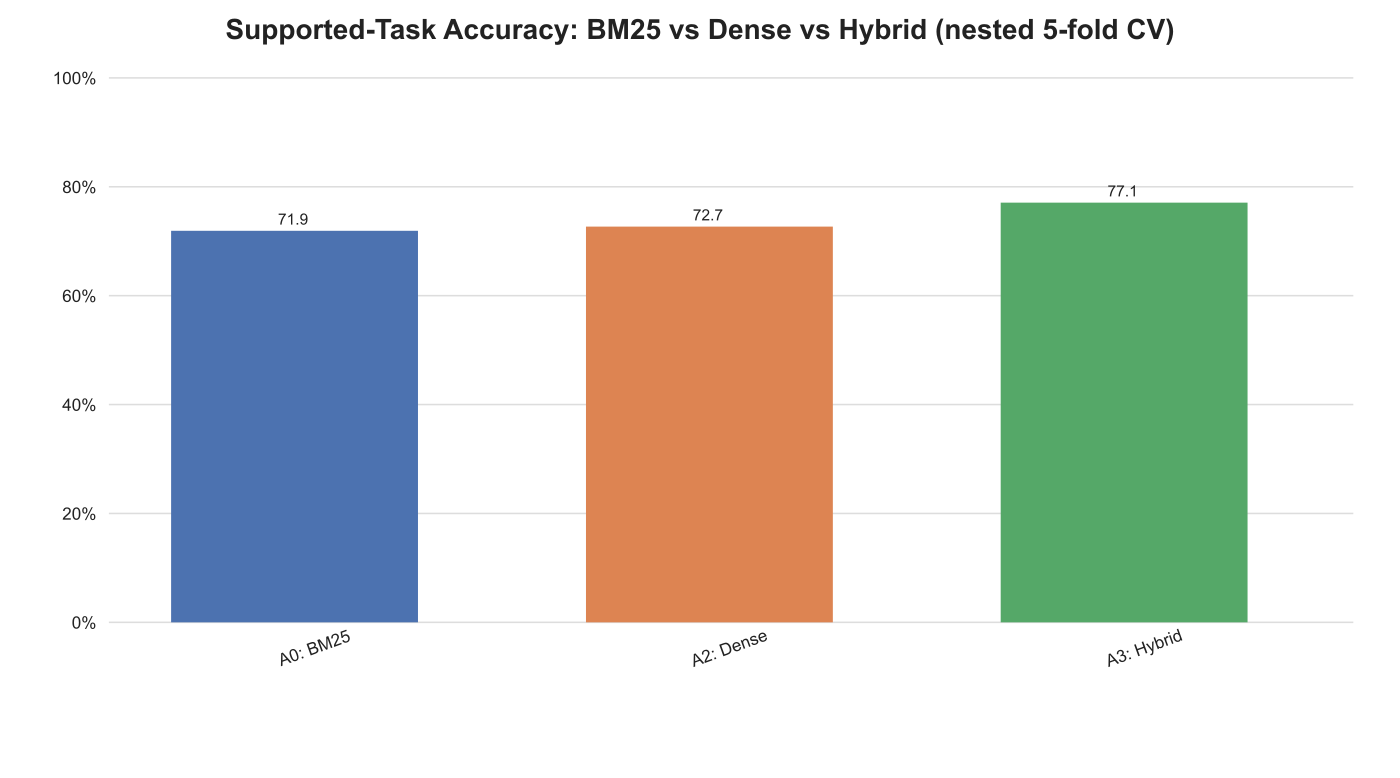
\includegraphics[width=0.48\linewidth]{figures/fig1_baseline_vs_improved_accuracy.png} \hfill
  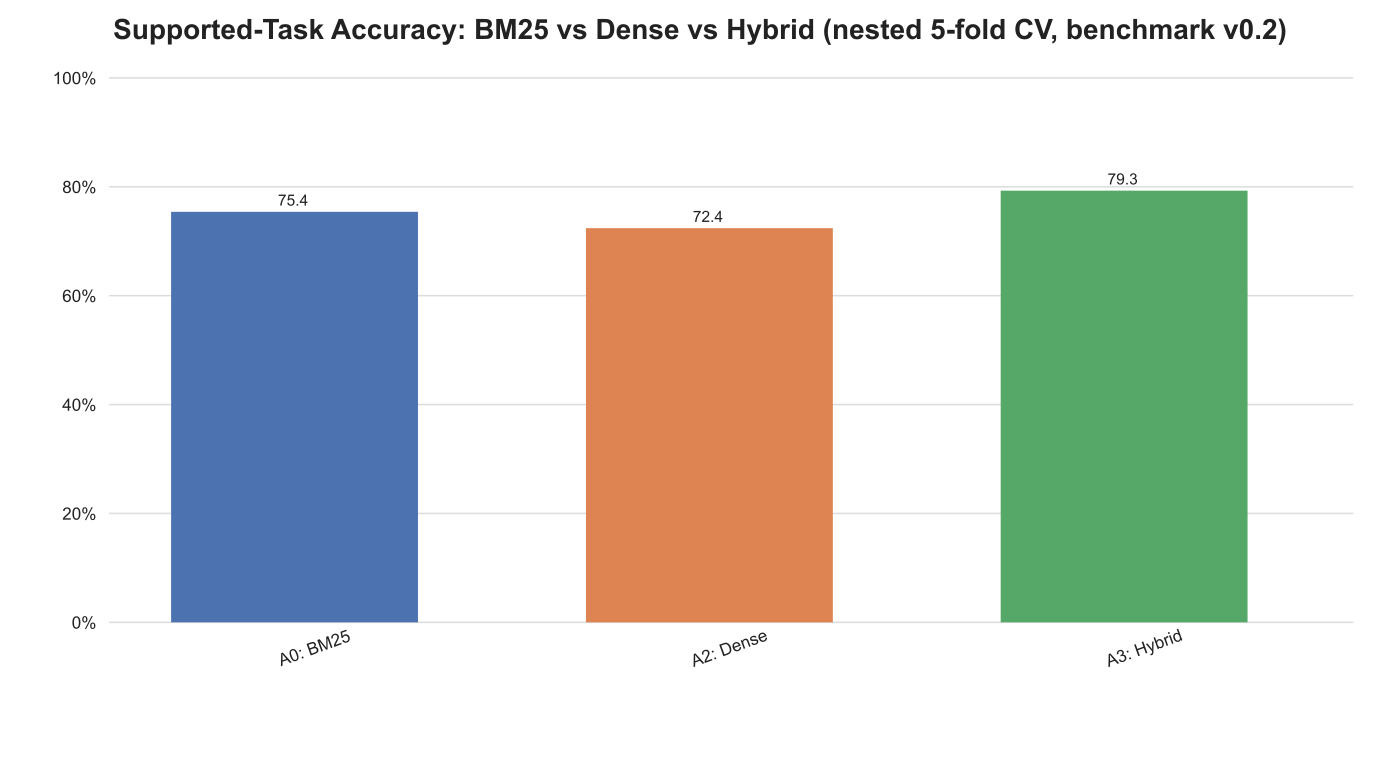
\includegraphics[width=0.48\linewidth]{figures/fig1_baseline_vs_improved_accuracy_v0.2.png}
  \caption{Accuracy on non-OOD queries (pooled; $n=135$ and $159$, including the 25 canonical controls) for BM25,
  dense-only, and hybrid retrieval. Left: v0.1. Right: v0.2.}
  \label{fig:accuracy}
\end{figure*}

\begin{figure*}[t]
  \centering
  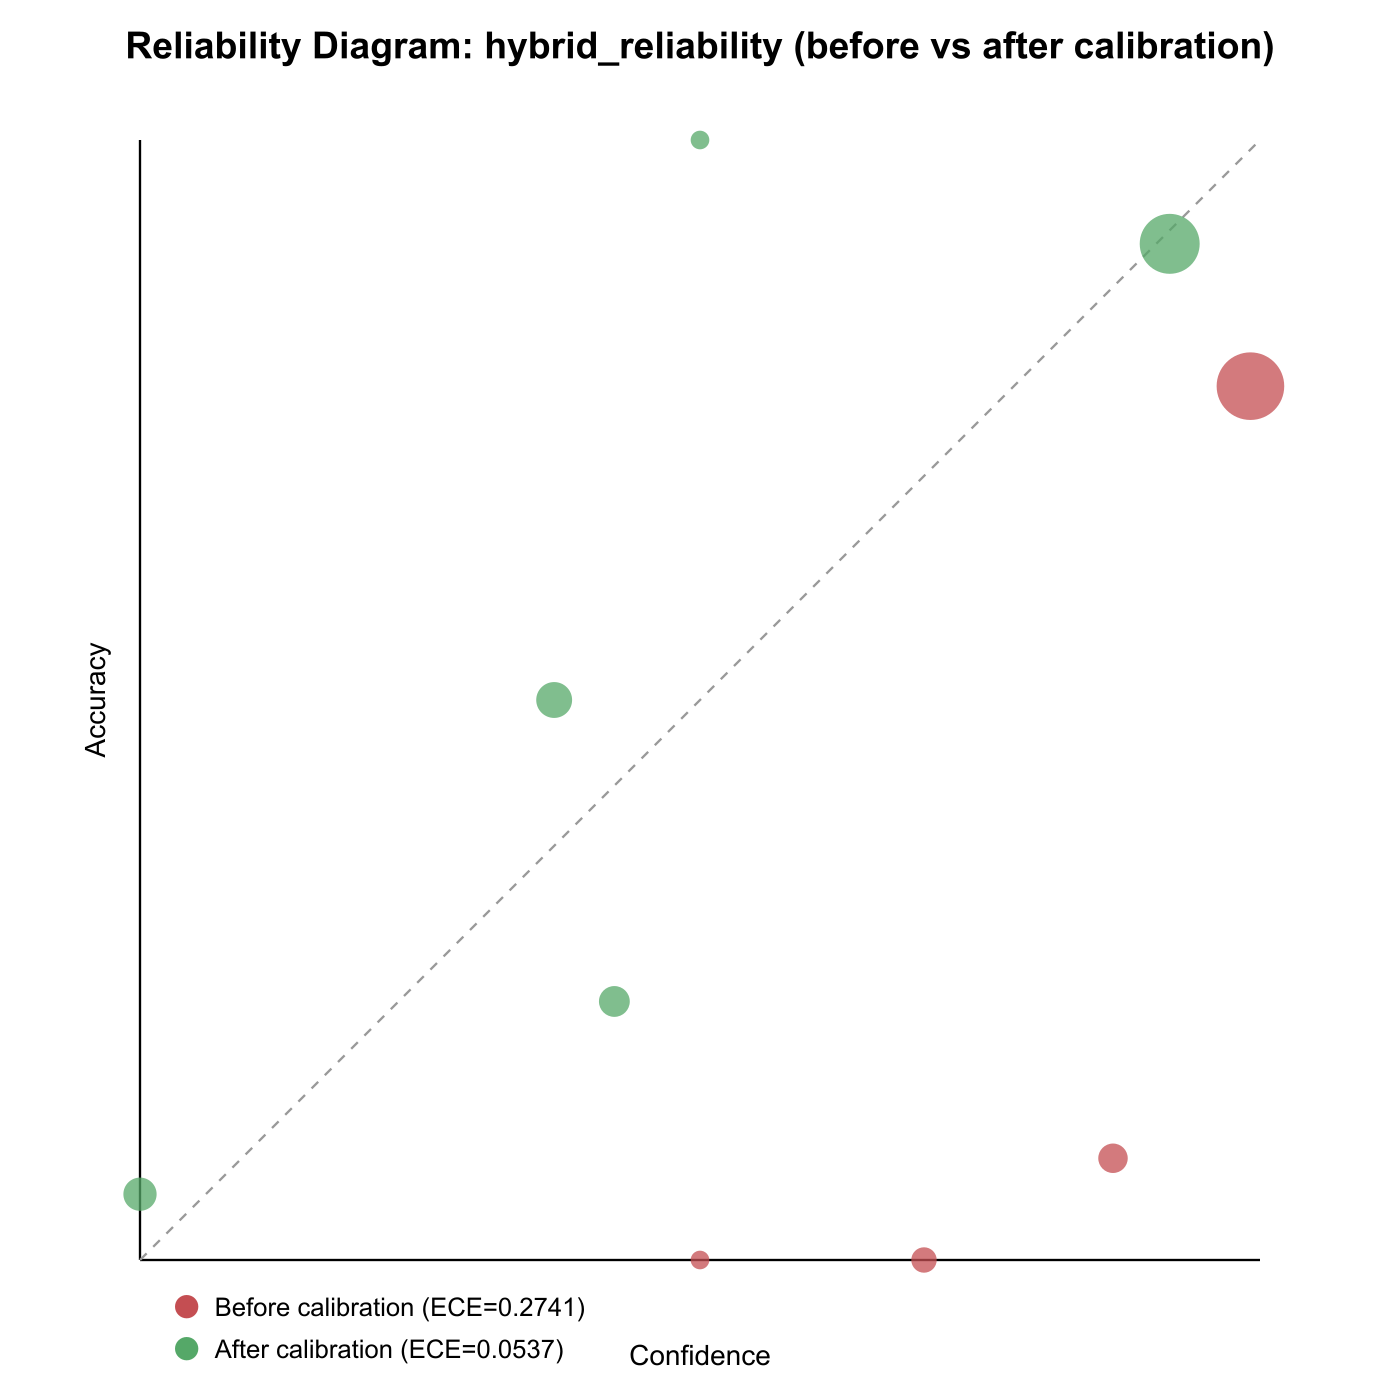
\includegraphics[width=0.40\linewidth]{figures/fig3_reliability_diagram.png} \hspace{0.08\linewidth}
  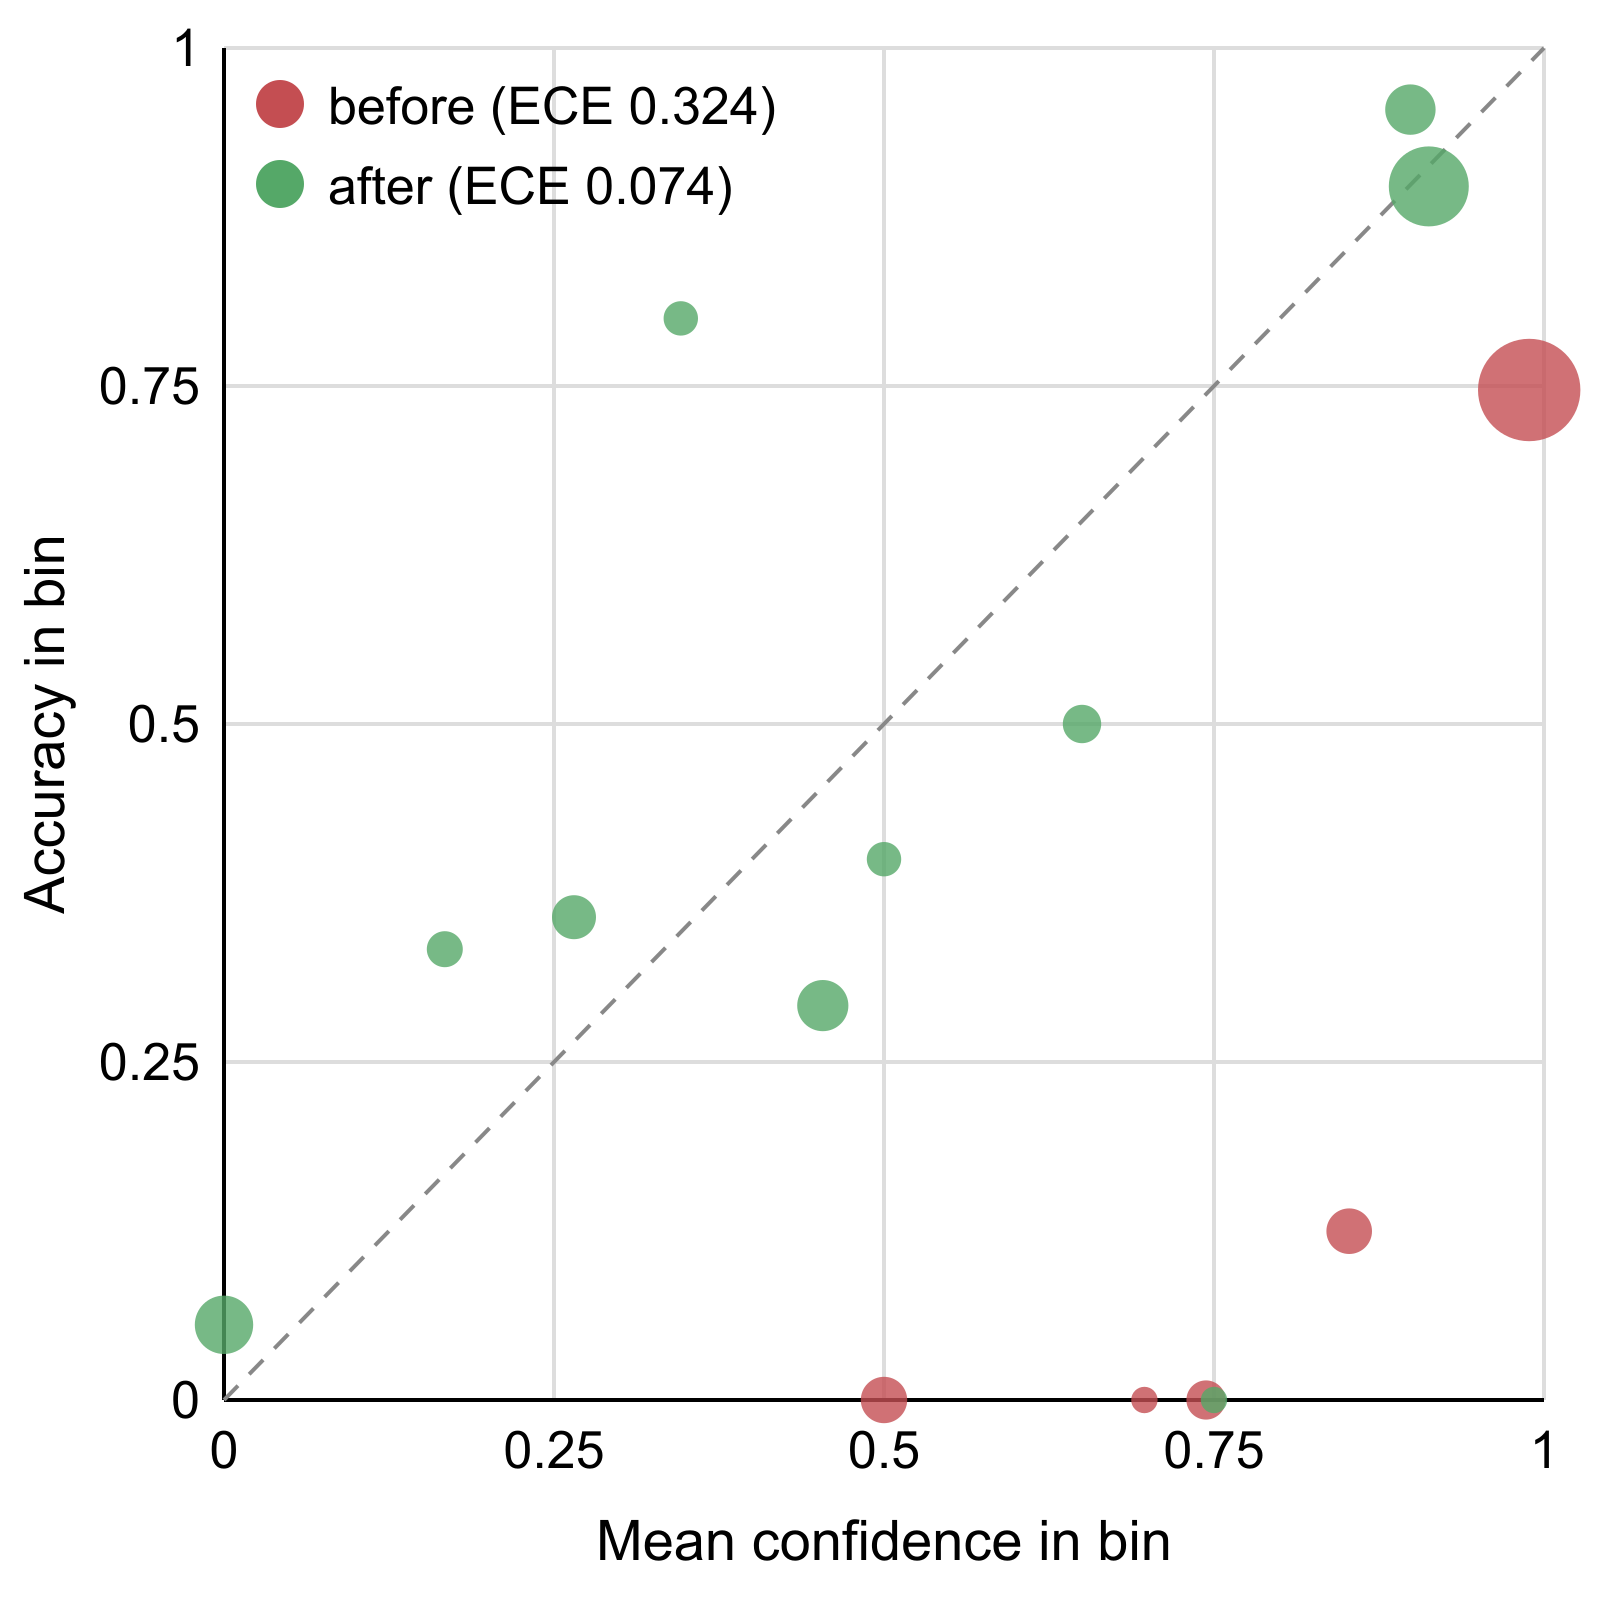
\includegraphics[width=0.40\linewidth]{figures/fig3_reliability_diagram_v0.2.png}
  \caption{Reliability diagram for the hybrid system's fused-score confidence, before vs.\ after isotonic calibration
  (10 equal-width bins; dot area grows with the number of predictions; dashed line: perfect calibration). Left: v0.1.
  Right: v0.2.}
  \label{fig:reliability}
\end{figure*}

\begin{figure*}[t]
  \centering
  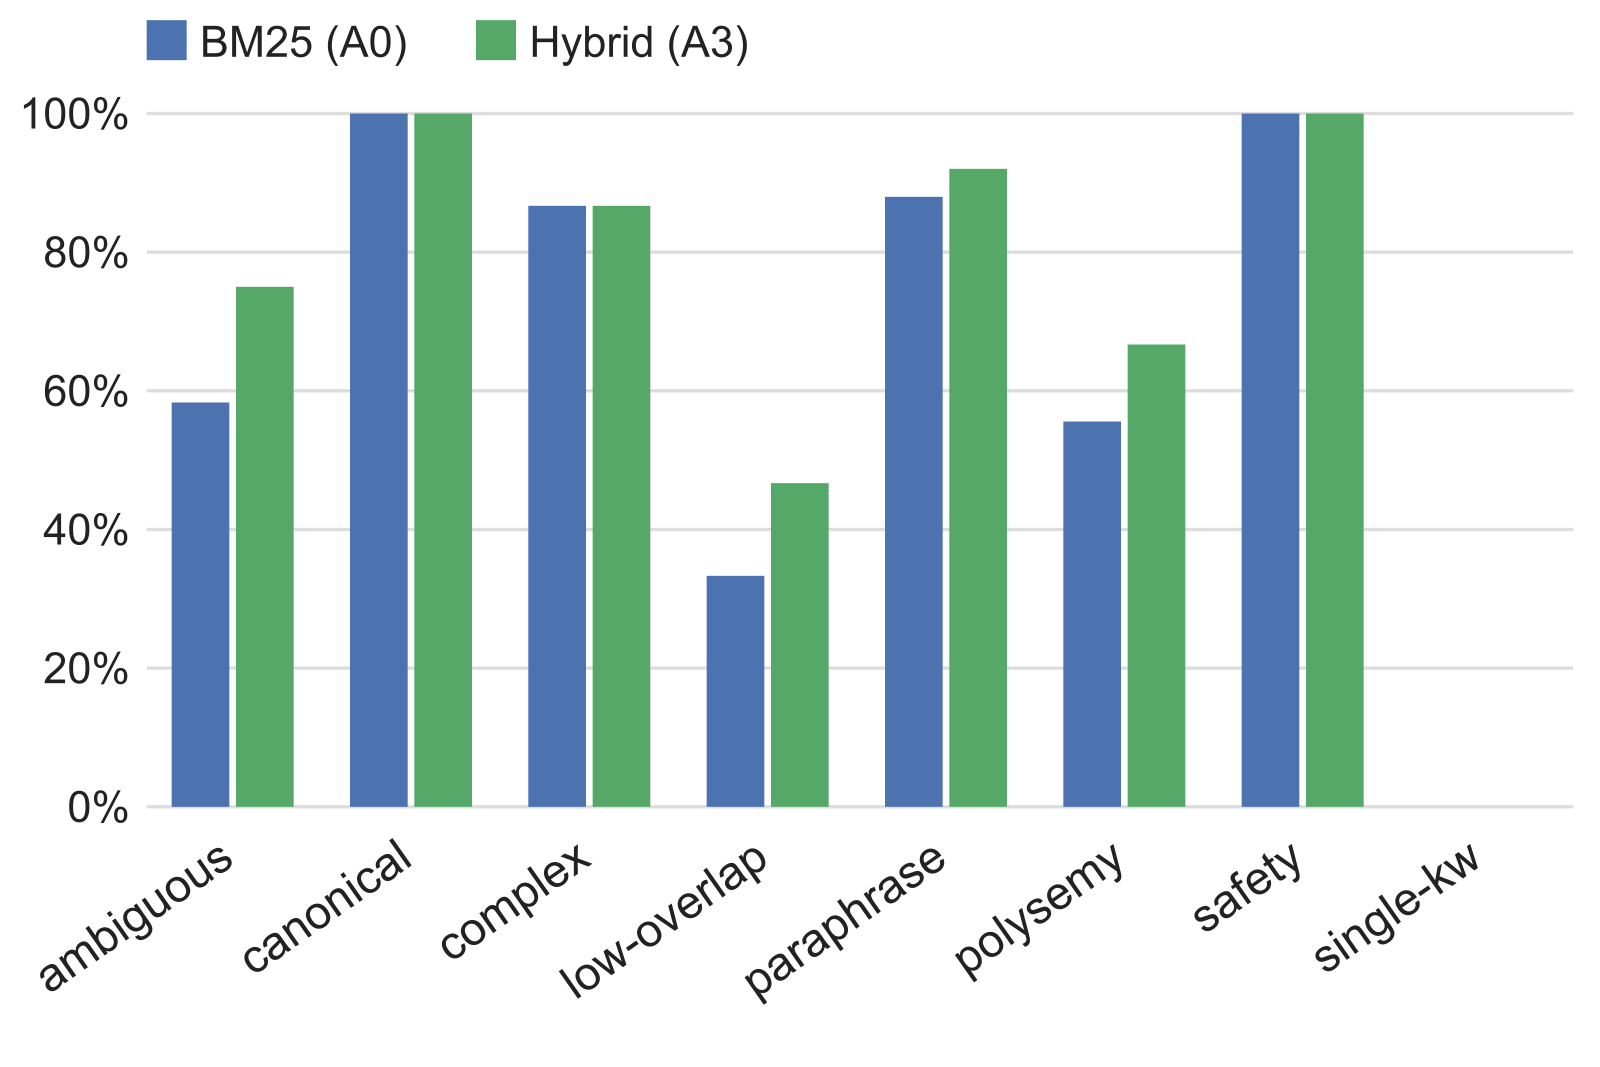
\includegraphics[width=0.48\linewidth]{figures/fig2_accuracy_by_query_type.png} \hfill
  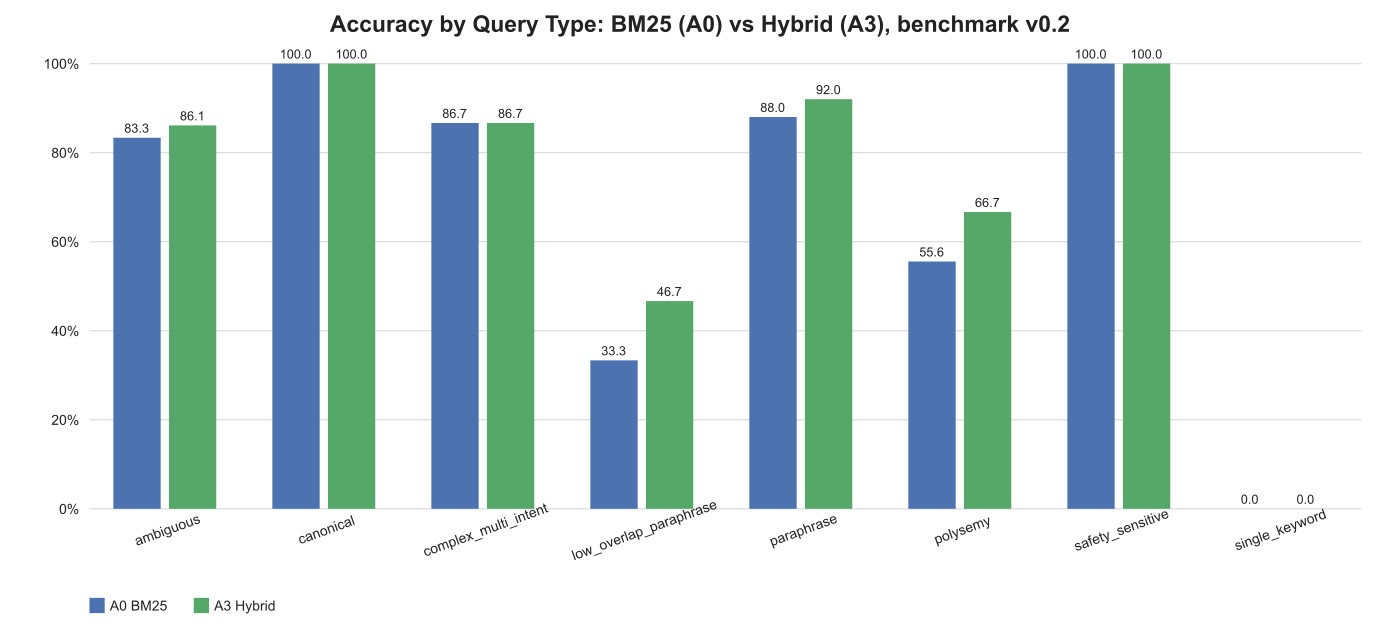
\includegraphics[width=0.48\linewidth]{figures/fig2_accuracy_by_query_type_v0.2.png}
  \caption{Accuracy by query type, BM25 (A0) vs.\ hybrid (A3). Single-keyword queries are 0\% for both systems, so
  their bars are empty. Left: v0.1. Right: v0.2.}
  \label{fig:bytype}
\end{figure*}

\begin{figure*}[t]
  \centering
  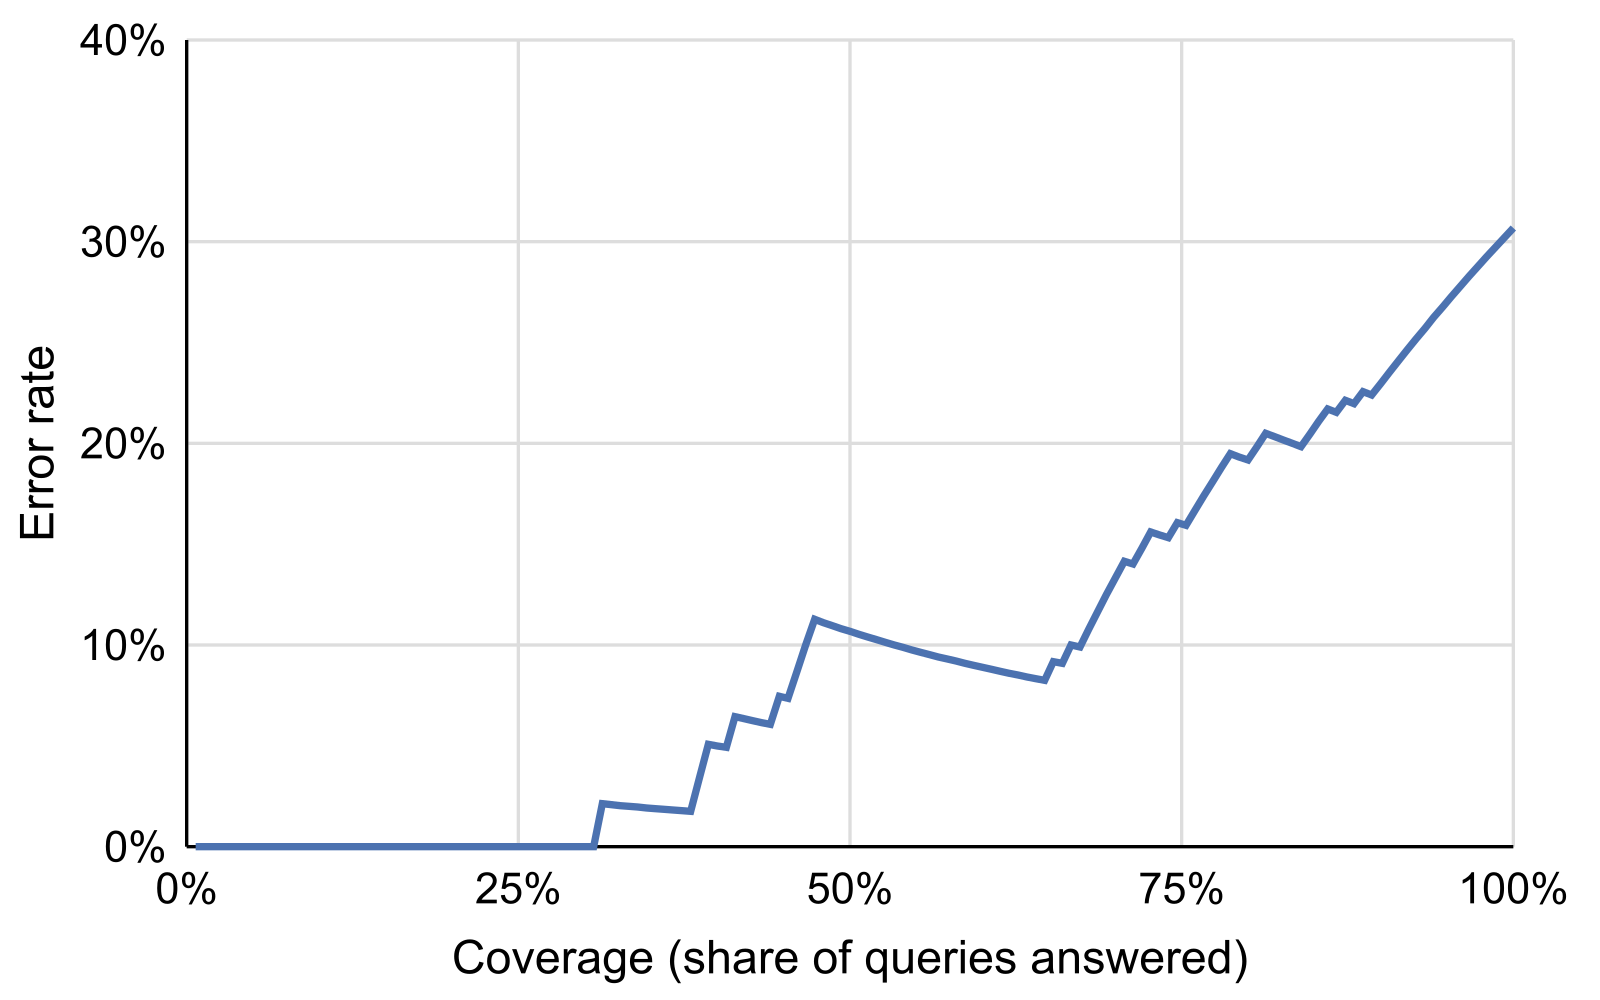
\includegraphics[width=0.48\linewidth]{figures/fig4_risk_coverage_curve.png} \hfill
  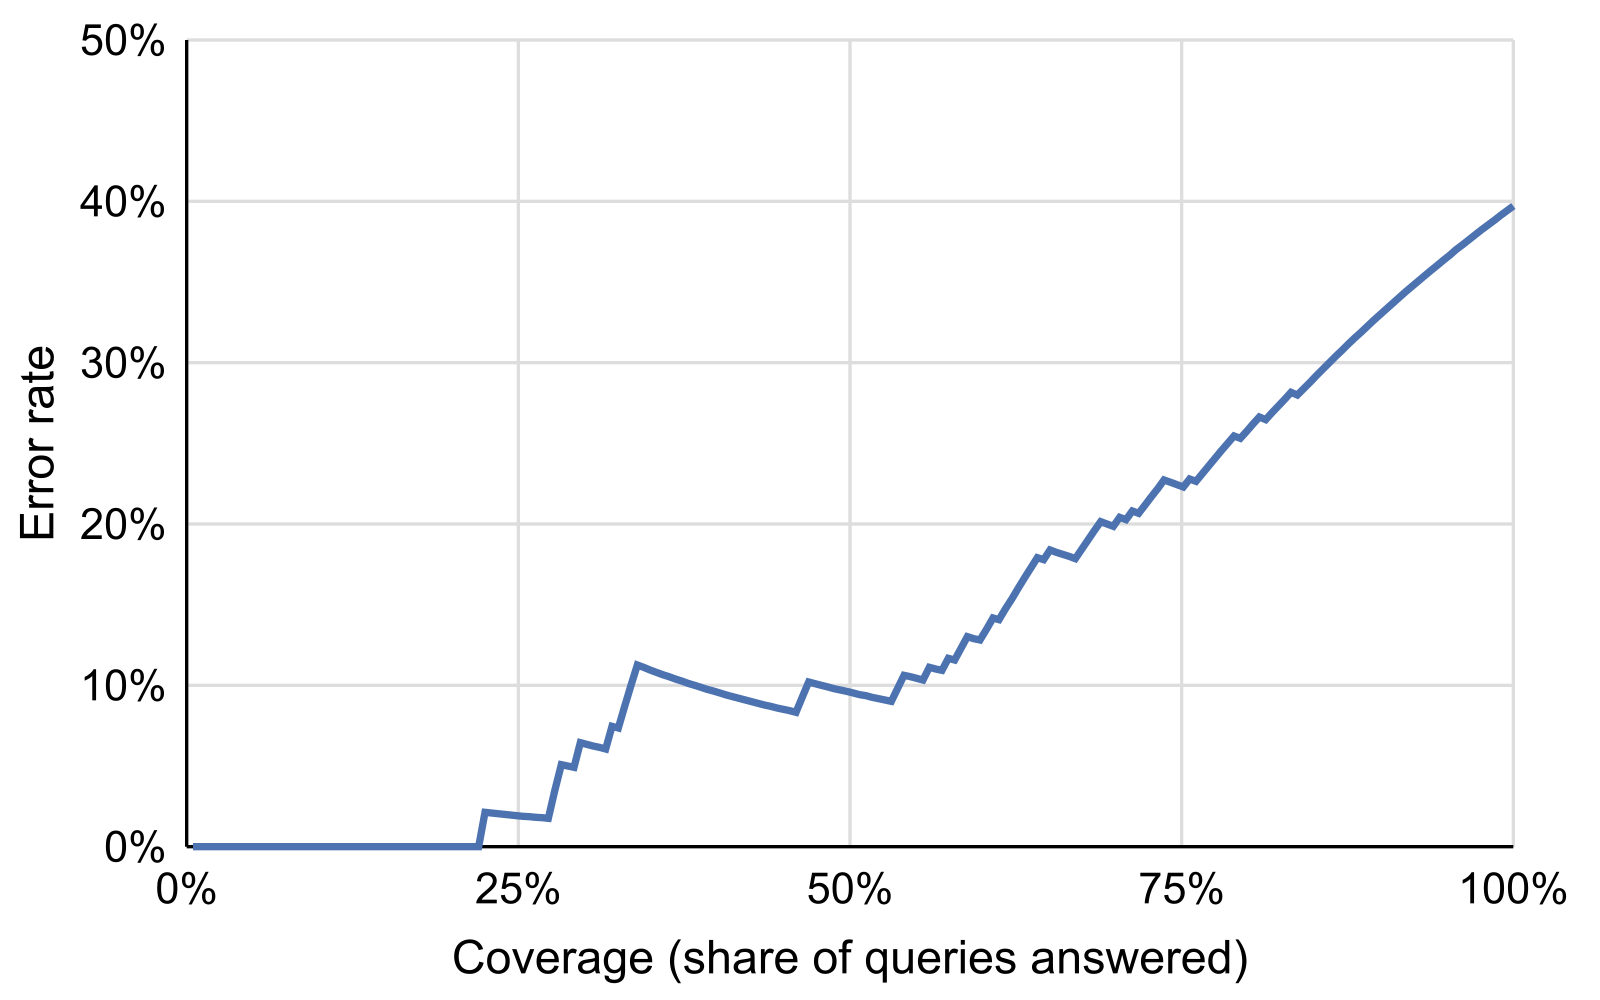
\includegraphics[width=0.48\linewidth]{figures/fig4_risk_coverage_curve_v0.2.png}
  \caption{Risk-coverage curve for the hybrid system: queries are answered in order of decreasing confidence, and the
  error rate is computed over the answered share. Tied confidences are answered in benchmark order, so points inside
  a tie block depend on that order; tie-aware values are in the text. Left: v0.1. Right: v0.2.}
  \label{fig:riskcoverage}
\end{figure*}

\begin{figure*}[t]
  \centering
  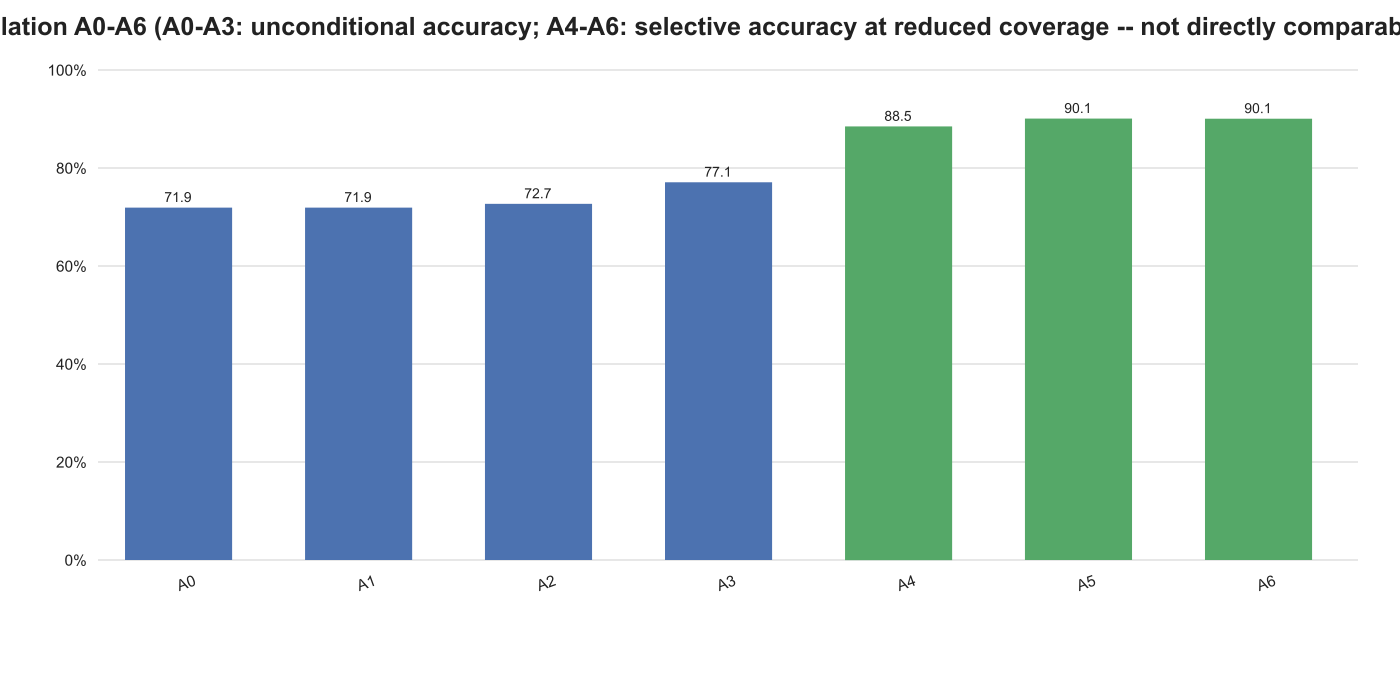
\includegraphics[width=0.48\linewidth]{figures/fig5_ablation_A0_A6.png} \hfill
  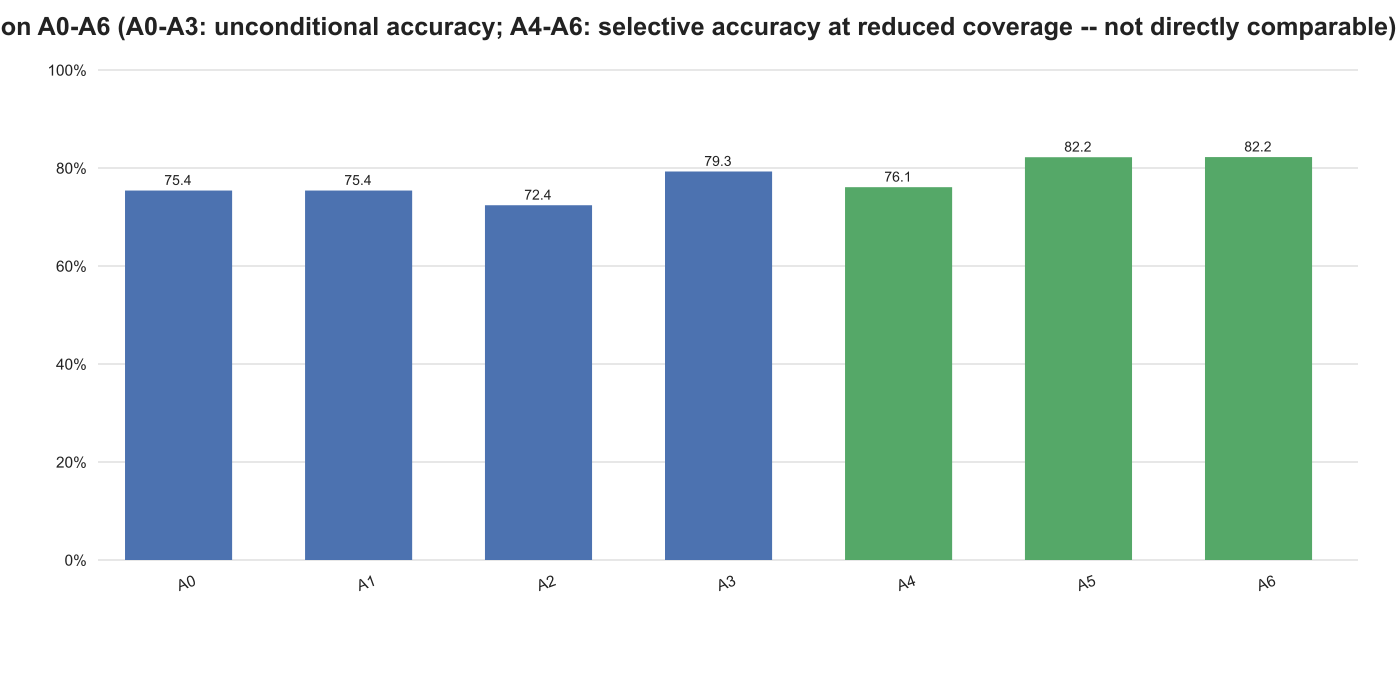
\includegraphics[width=0.48\linewidth]{figures/fig5_ablation_A0_A6_v0.2.png}
  \caption{Ablation A0--A6. A0--A3: accuracy on all non-OOD queries (pooled). A4--A6: selective accuracy on the queries
  each configuration answers (mean over folds), at reduced coverage, so not directly comparable to A0--A3. Left: v0.1.
  Right: v0.2.}
  \label{fig:ablation}
\end{figure*}
